\documentclass[10pt,a4paper]{article}
\usepackage[margin=0.65in]{geometry}
\usepackage{amsmath,booktabs,graphicx,float}
\title{Breast Tumour Classification Using a NumPy Neural Network}
\author{CS4152 -- Deep Learning and Neural Networks\\Names and Roll Numbers: \textit{Add both group members}}
\date{Fall 2026}
\begin{document}
\maketitle
\section{Data and Model}
The Wisconsin Diagnostic Breast Cancer dataset has 569 samples and 30 numerical features. We used a stratified 70/15/15 split with seed 42, giving 398 training, 85 validation, and 86 test samples. Standardization used only training-set means and standard deviations; using held-out data would leak information and bias evaluation.

The MLP architecture was $30$--$16$--$8$--$1$, with ReLU hidden activations, sigmoid output, He-normal weight initialization, and zero biases. It has
\[
(30\cdot16+16)+(16\cdot8+8)+(8\cdot1+1)=641
\]
trainable parameters. Forward/backward passes, binary cross-entropy, SGD, momentum, RMSprop, and Adam were implemented in NumPy, with mini-batches of 32.

\section{Gradient Check}
Central differences were computed as
\[
g_i^{(n)}=\frac{L(\theta_i+\epsilon)-L(\theta_i-\epsilon)}{2\epsilon},
\quad \epsilon=10^{-5}.
\]
The relative error was $2.5531\times10^{-11}$, below the required $10^{-6}$ threshold.

\section{Optimizer and Learning-Rate Experiments}
Table~\ref{tab:opt} gives losses after 150 epochs. Validation loss is unregularized binary cross-entropy.
\begin{table}[H]\centering
\caption{Optimizer comparison after 150 epochs}\label{tab:opt}
\begin{tabular}{lrr}\toprule Optimizer & Training loss & Validation loss\\\midrule
SGD ($\eta=0.01$) & 0.0559 & 0.1010\\
Momentum ($\eta=0.01$) & 0.0029 & 0.2927\\
RMSprop ($\eta=0.001$) & 0.0003 & 0.4365\\
Adam ($\eta=0.001$) & 0.0040 & 0.2393\\\bottomrule
\end{tabular}
\end{table}
Momentum and adaptive optimizers reduce training loss quickly, but validation loss rises, indicating overfitting. SGD had the lowest validation loss at epoch 150 in this run.
\begin{figure}[H]\centering
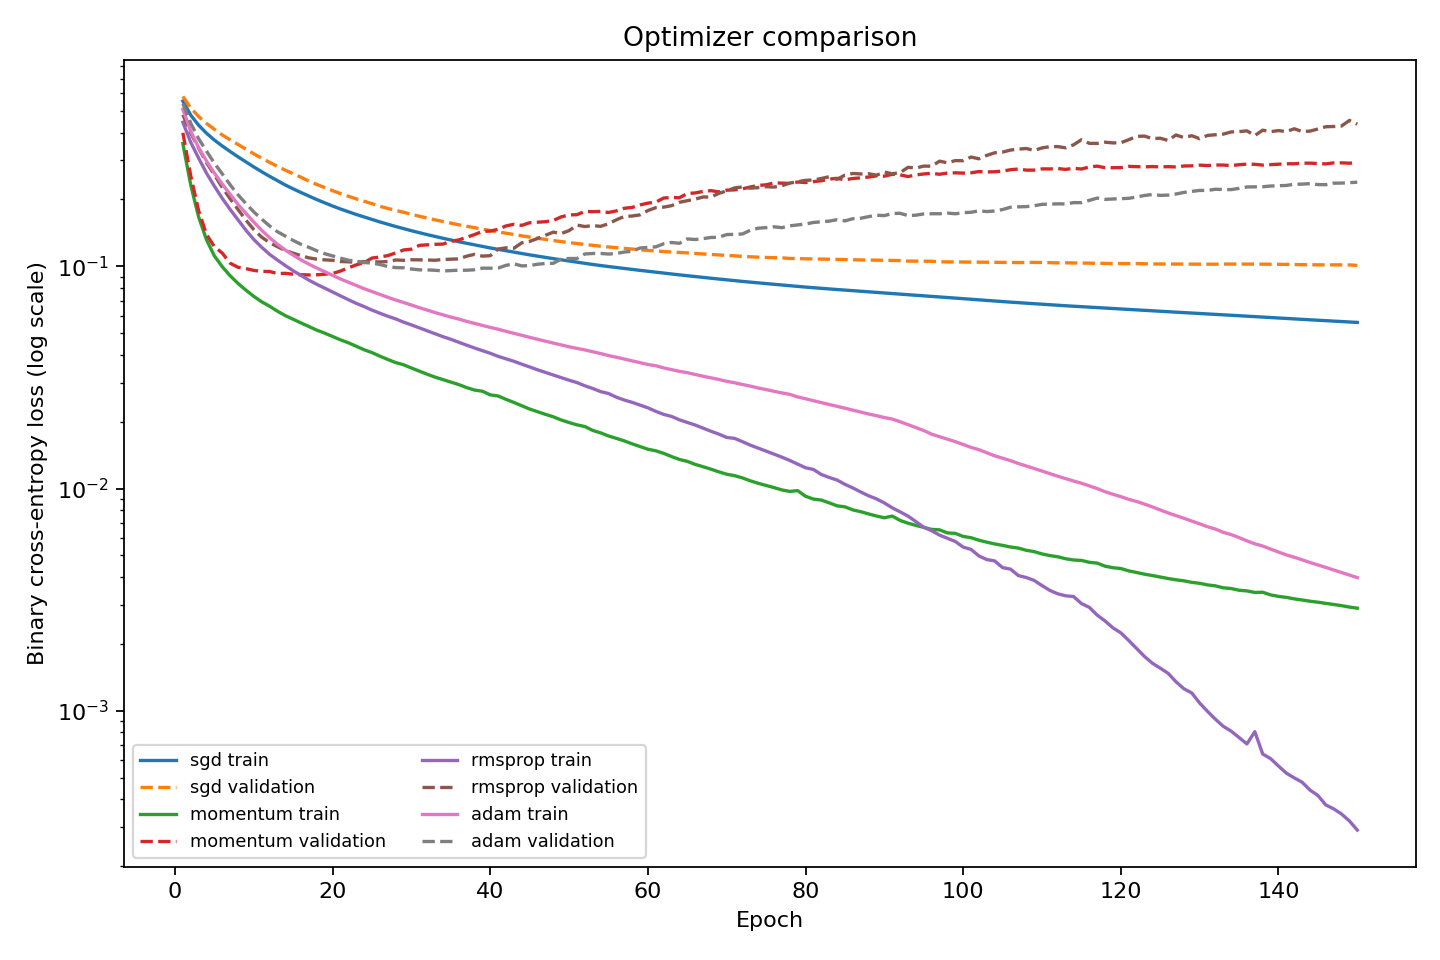
\includegraphics[width=0.82\linewidth]{q5_optimizers.png}
\caption{Training and validation loss for four optimizers (log scale).}
\end{figure}

For learning rates $10^{-4},10^{-3},10^{-2},10^{-1},1$, final training/validation losses were respectively 0.5134/0.5460, 0.2233/0.2612, 0.0559/0.1010, 0.0029/0.3062, and 0.0001/0.4986. A very small rate learns slowly; a large rate can fit the training set quickly but generalize poorly.
\begin{figure}[H]\centering
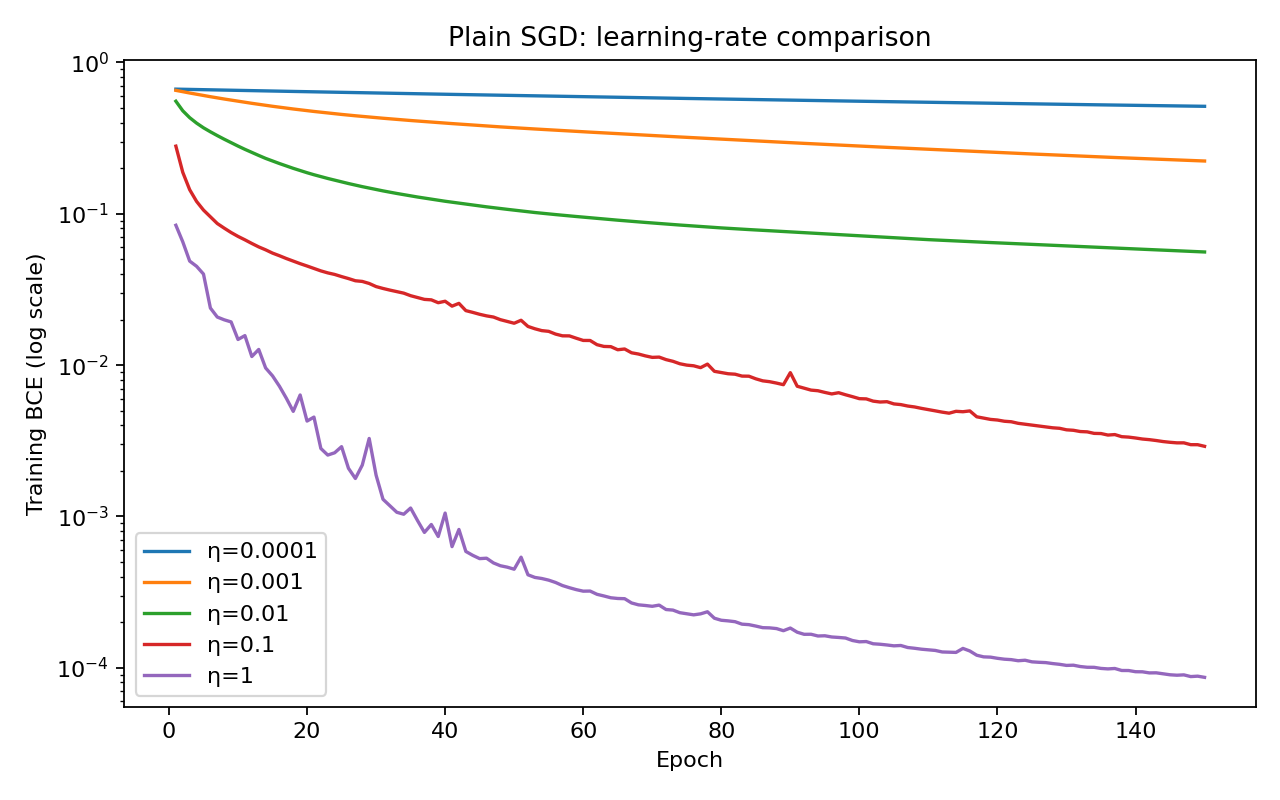
\includegraphics[width=0.72\linewidth]{q5_learning_rates.png}
\caption{Plain SGD training loss for different learning rates (log scale).}
\end{figure}

\section{Regularization and Evaluation}
Adam with L2 used $\lambda=0.01$ and penalty $\frac{\lambda}{2}\sum W^2$. Early stopping used patience 20 and restored the best validation weights.
\begin{table}[H]\centering
\caption{Regularization comparison}\label{tab:reg}
\begin{tabular}{lrrr}\toprule Method & Training objective & Validation loss & $\|W\|_F$\\\midrule
None & 0.0001 & 0.3832 & 9.7389\\
L2 & 0.0869 & 0.1104 & 3.3928\\
L2 + early stopping & 0.1607 & 0.0851 & 4.6843\\\bottomrule
\end{tabular}
\end{table}
L2 objectives include the penalty, while validation losses do not. Without regularization the model overfits (high variance); L2 shrinks weights, and early stopping limits overfitting. Their combination had the best validation loss.

The selected L2 + early-stopping model achieved test accuracy 98.84\%, precision 100.00\%, recall 96.88\%, and F1-score 98.41\%. With malignant as positive, the confusion matrix (actual rows: benign, malignant; predicted columns: benign, malignant) was
\[
\begin{bmatrix}54&0\\1&31\end{bmatrix}.
\]
A false negative (malignant classified as benign) is generally more costly because it can delay treatment. Lowering the threshold usually increases malignant recall but may increase false positives; choose the threshold using validation data, not test data.

\section{Conclusion}
The gradient check passed and regularization improved validation performance. These results apply to this split and configuration; clinical deployment would require broader validation and expert oversight.
\end{document}
